\section{Service}\label{service}

A convenient Web service is included in Cloudmesh cc. It allows the user
to manage and visualize the status of workflows through a Web browser
interface. At this time the focus is that the interface can be run by a
singleuser on the local machine. This allows that remote executions of
workflow nodes run completely independent from cloudmesh cc and
interaction is possible in asynchronous mode.

\subsection{Management}\label{management}

To start the service use the command:

\begin{verbatim}
cms cc start
\end{verbatim}

For debugging purposes with outoreload on code changes, you can use the
command:

\begin{verbatim}
cms cc start --reload
\end{verbatim}

To stop the service use the command:

\begin{verbatim}
cms cc stop
\end{verbatim}

To view the interface to the service use the command:

\begin{verbatim}
cms cc view
\end{verbatim}

\subsection{Example Workflow}\label{example-workflow}

An example workflow can be generated by clicking on the Example
sidebar menu.

\subsection{Table View}\label{table-view}

The workflow can then be viewed while clicking on the workflow name
listed in the sidebar under workflows. Other workflows can be uploaded
and multiple workflows can be managed. Management buttons for the
workflow are included in this view.

\begin{figure}
\centering
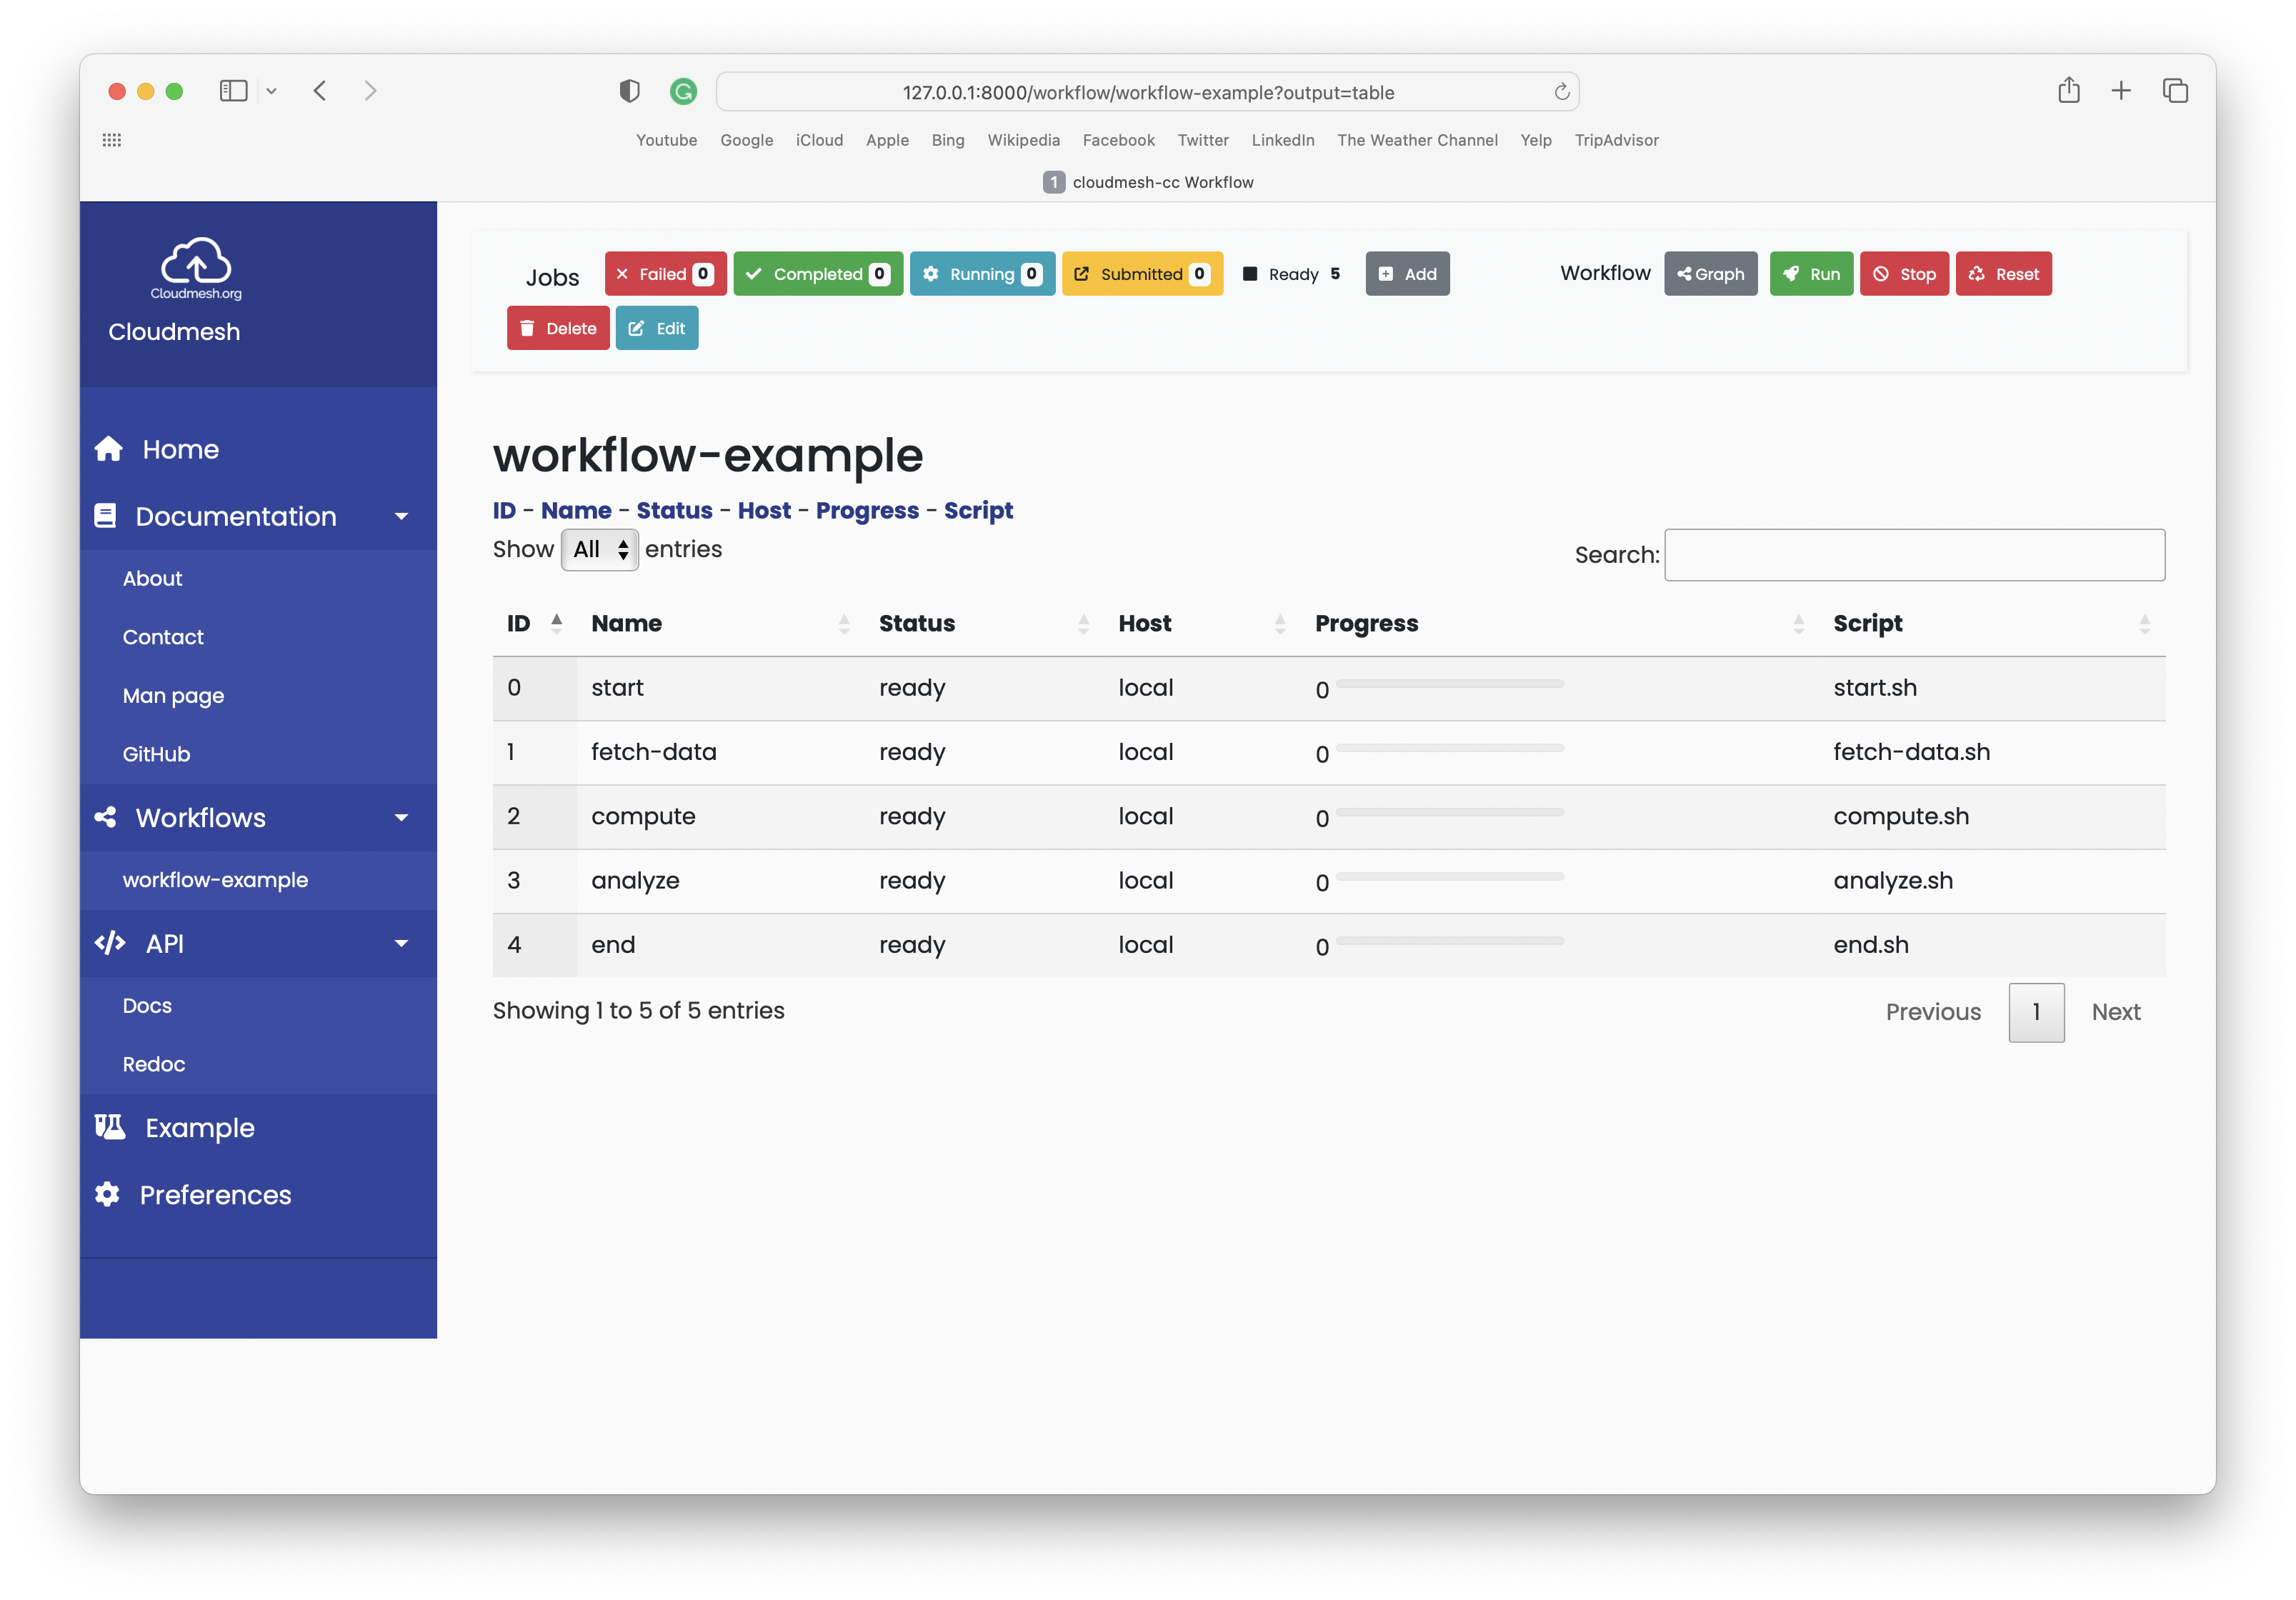
\includegraphics[width=1.05\columnwidth]{images/service-table.png}
\caption{Cloudmesh cc workflow Table view}
\end{figure}

\subsection{Graph View}\label{graph-view}

One can switch back and forth between a graph and a table view while
using the included buttons, it will take a moment to update them.

\begin{figure}
\centering
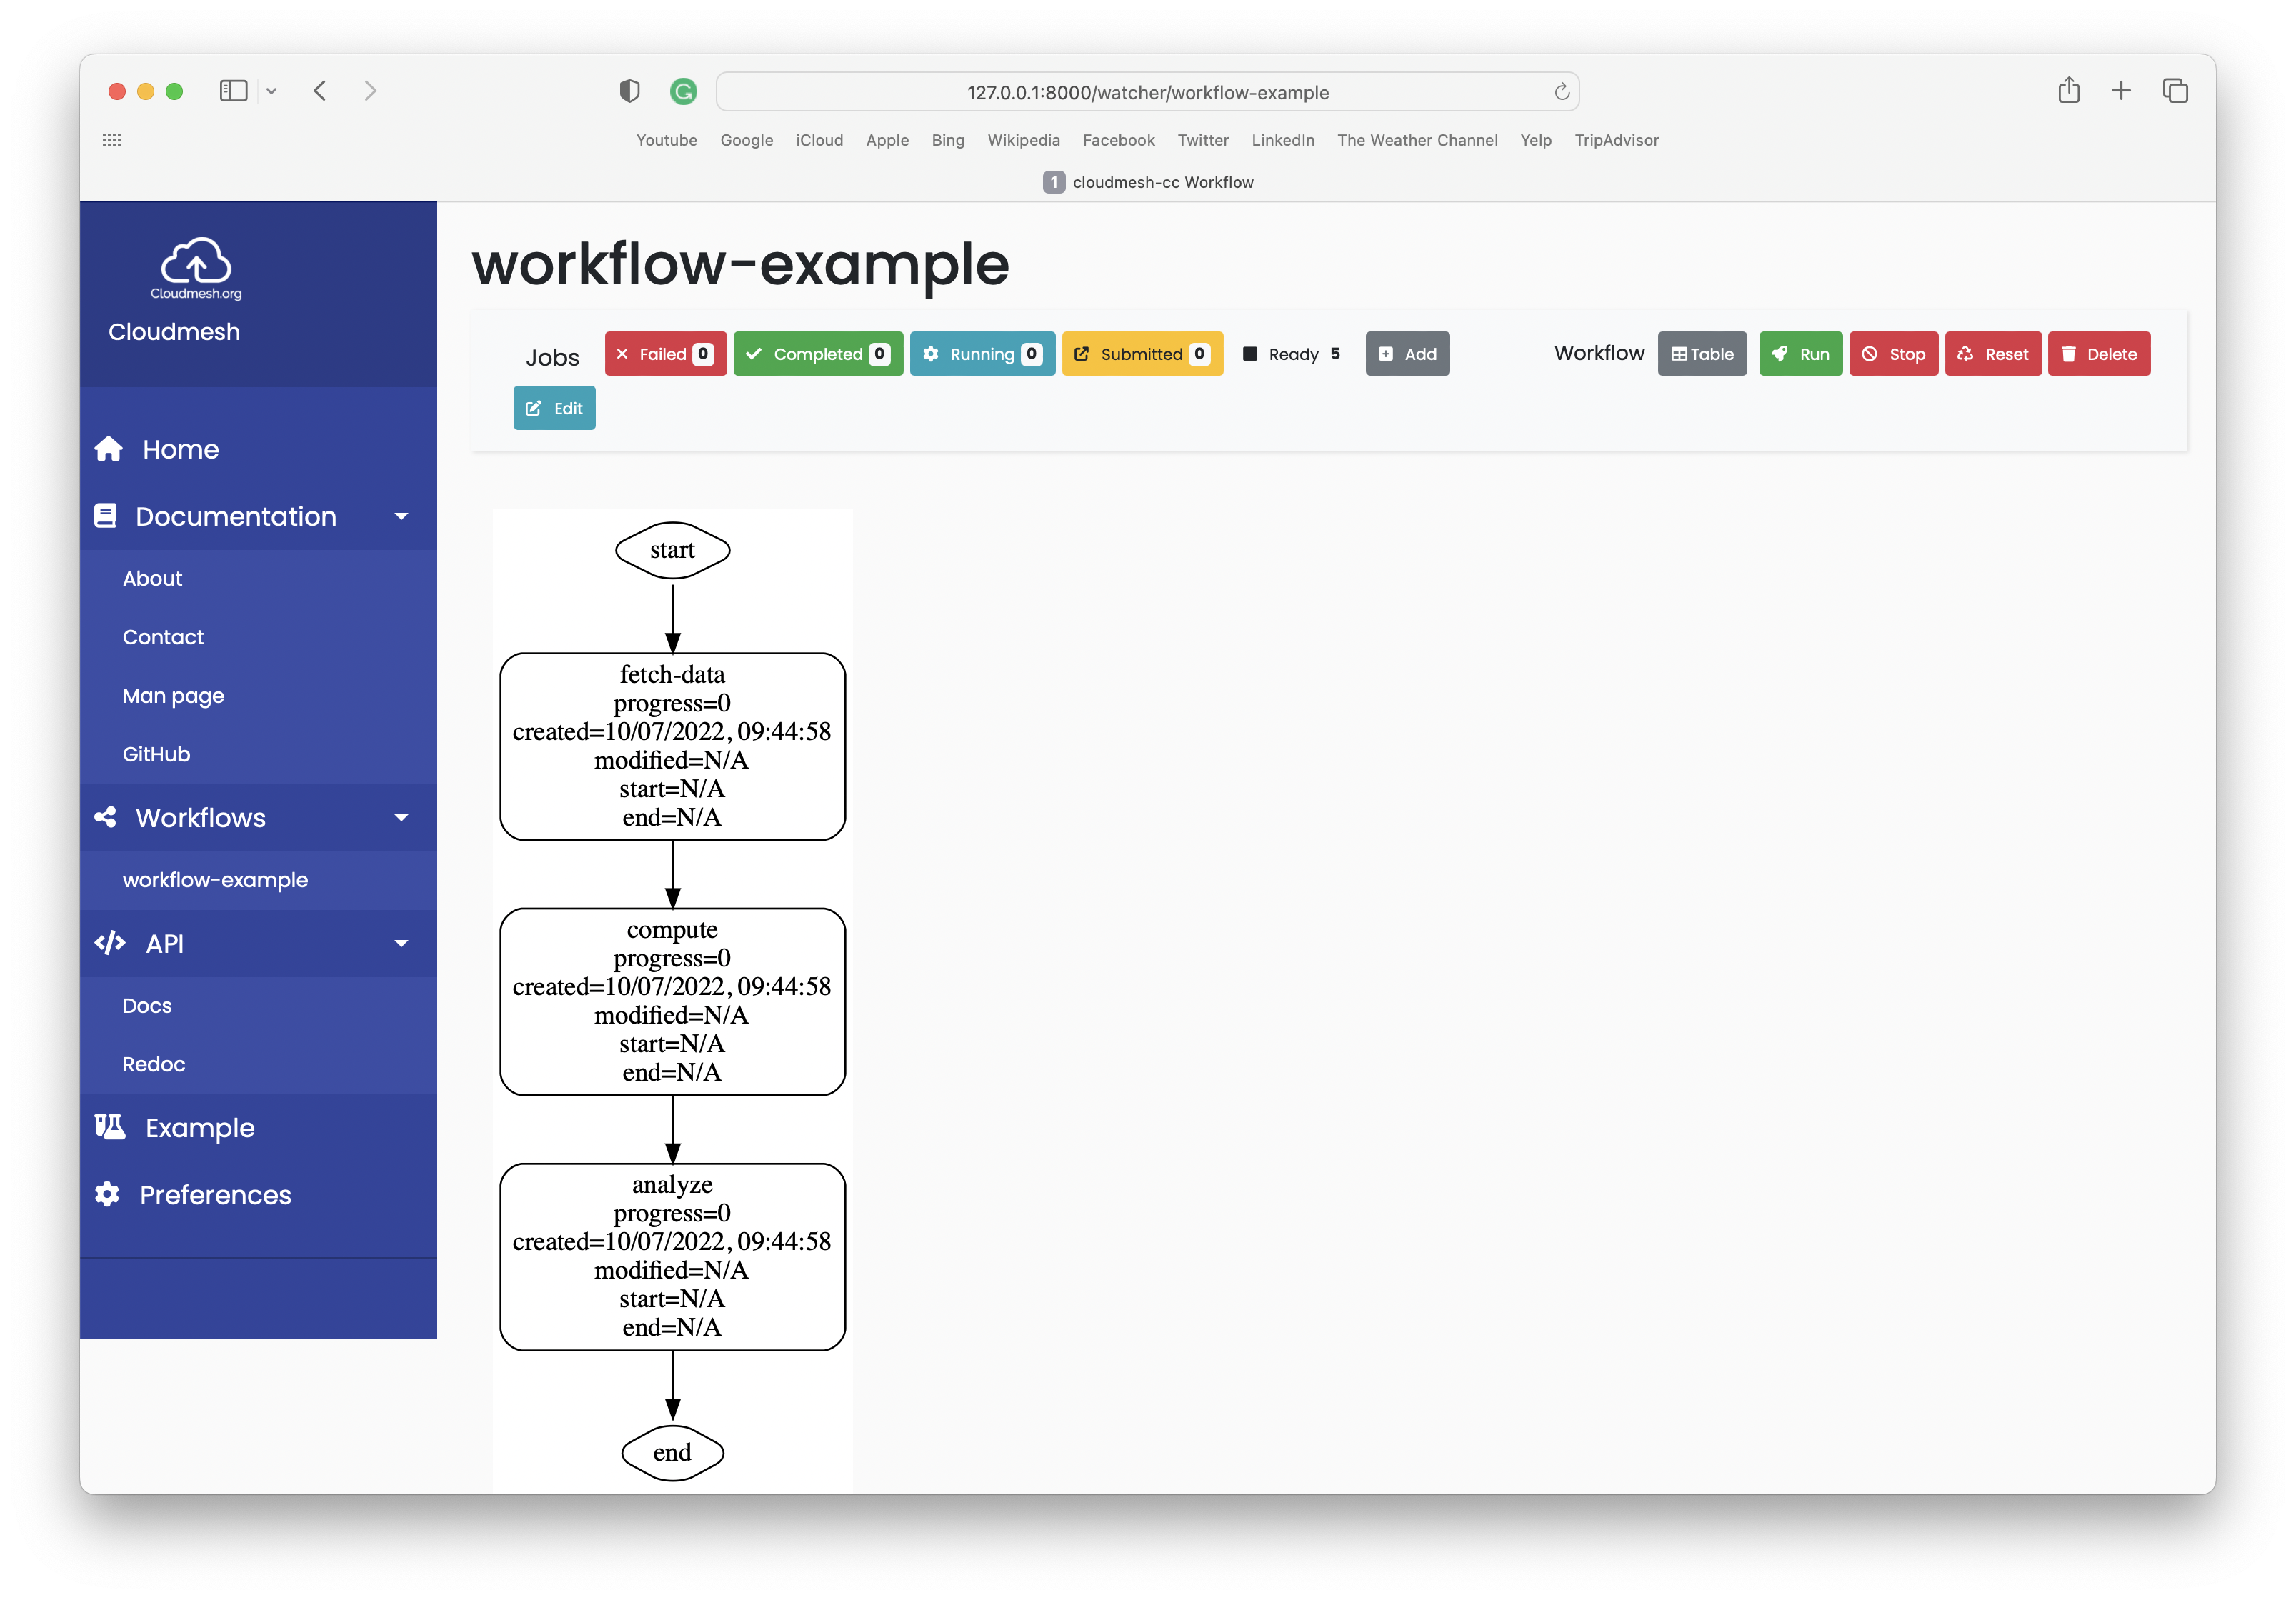
\includegraphics[width=1.05\columnwidth]{images/service-graph.png}
\caption{Cloudmesh cc workflow graph view}
\end{figure}
